%\documentclass[a4paper]{fhnwreport} %Legt grundlegende Formatierungen wie Schriftarten, Ort Seitenzahlen etc. fest.
%
%\graphicspath{{./graphics/}}%Change according to graphics folder!
%
%\begin{document}

\section{Software}
Die Anforderung des Auftraggebers beinhaltet, dass die Kommunikation zwischen Sensorplatine und Meldezentrale über die Powerline erfolgt oder keine zusätzliche Leitung beanspruchen darf. Für die drahtlose Übertragung war die Idee die Kommunikation über ein kabelloses System, wie Bluetooth oder Wireless zu verwenden. Diese Idee wurde aufgrund der unbekannten Distanzen zwischen der Sensor- und Meldeplatine verworfen. Die Kommunikation über die Powerline verlangt, dass die zu übertragenden Daten in diese im richtigen Format in die Leitung eingekoppelt wird. Für diese Einkopplung wird ein fertiger Transceiver und ein Kommunikationsprotokolls verwendet. Es wird auf der Sensorplatine ein ATMega328 verwendet.


\subsubsection{Sensorplatine}
Die Aufgabe der Sensorplatine basiert auf der Verarbeitung der gemessenen Daten zu übermittelbaren Daten. In der Abbildung \ref{fig:Software_Flussdiagramm_Sensorplatine} ist der Verlauf dieser Verarbeitung ersichtlich.

\begin{figure}[htbp] 
  \centering
     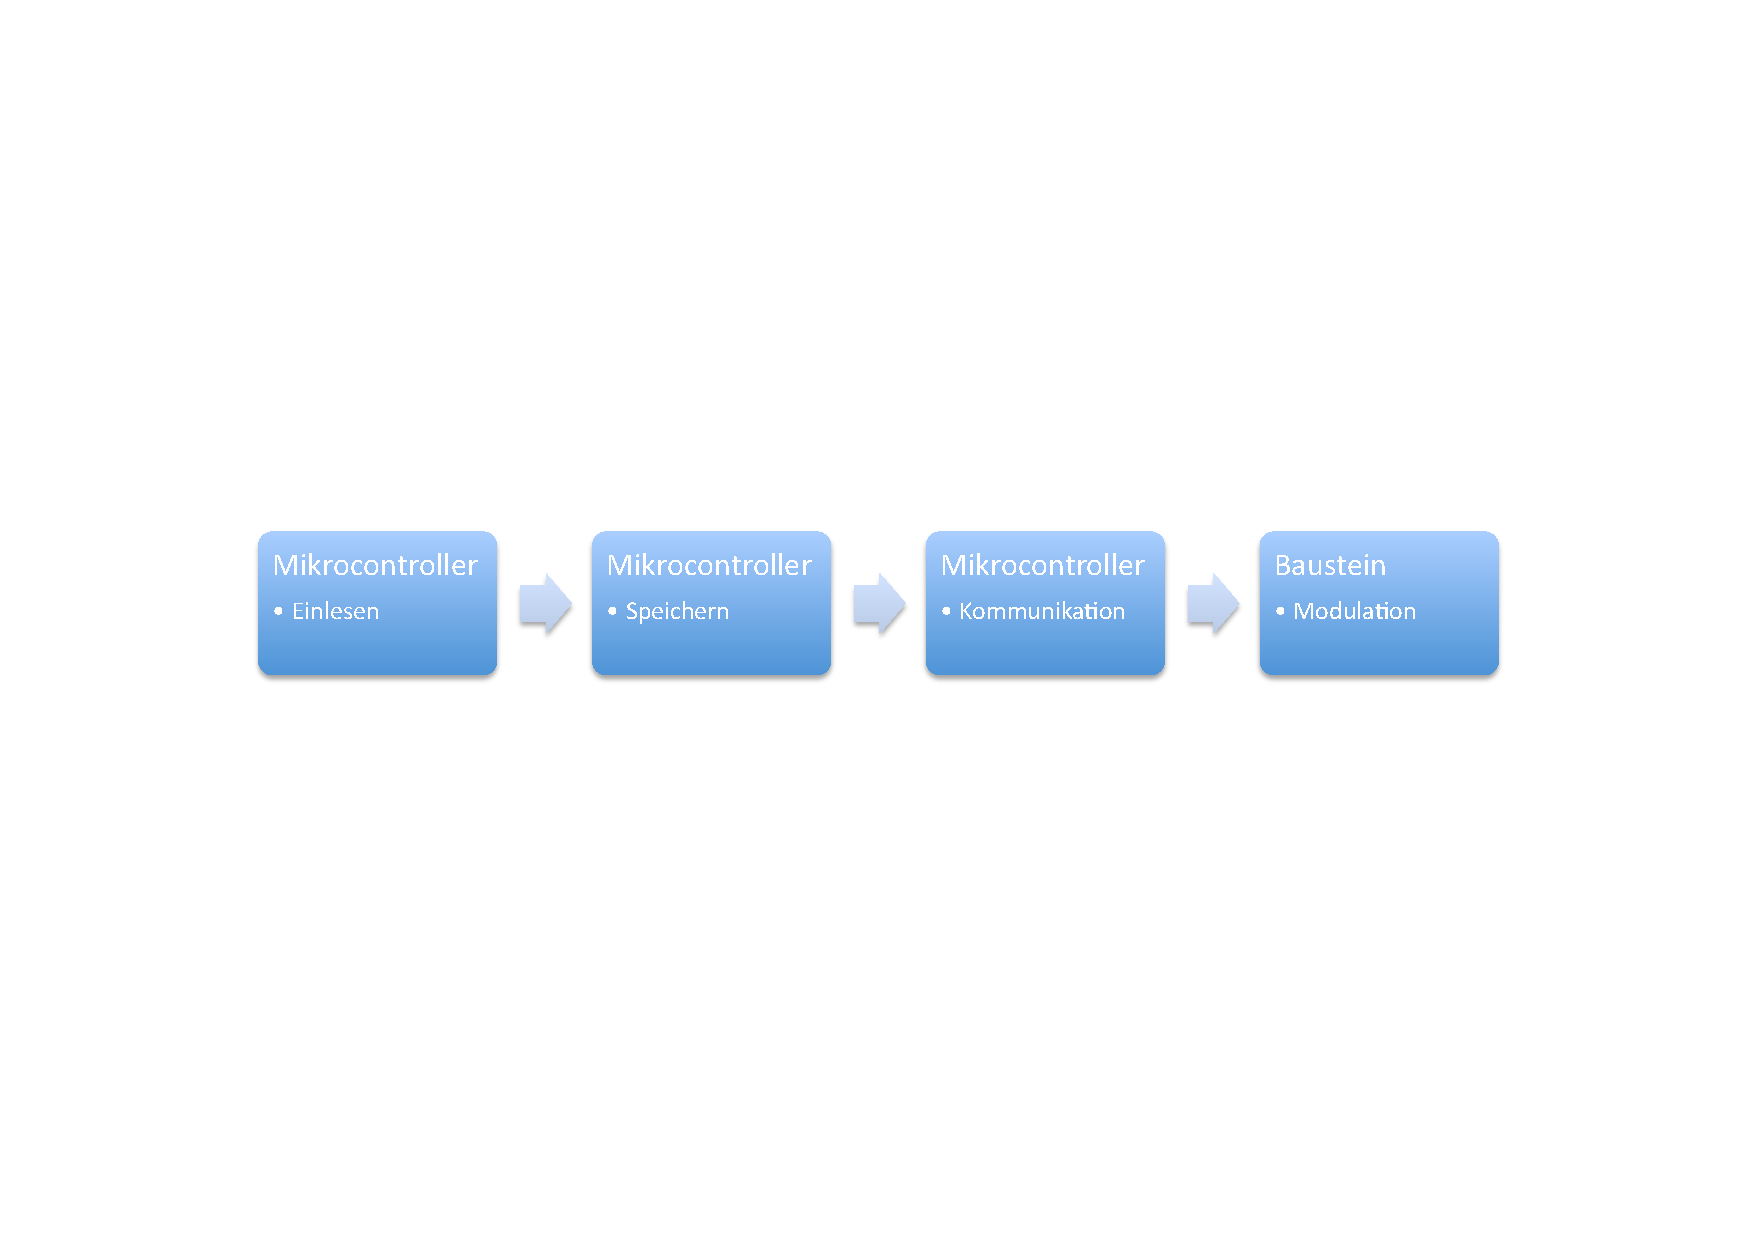
\includegraphics[width=1\textwidth]{graphics/Software_Flussdiagramm_Sensorplatine}
  \caption{Flussdiagramm Verlauf Programm Sensorplatine}
  \label{fig:Software_Flussdiagramm_Sensorplatine}
\end{figure}

Im ersten Schritt in der Abbildung \ref{fig:Software_Flussdiagramm_Sensorplatine} werden von der Messung die Daten eingelesen und in verwendbare Datentypen gespeichert. Die Kommunikation zum Transceiver wird über eine serielle asynchrone Schnittstelle stattfinden. \\Der Modulator wird die Messdaten auf die Leitung, Powerline Communication, koppeln.

\subsubsection{Meldeplatine}


\begin{figure}[htbp] 
  \centering
     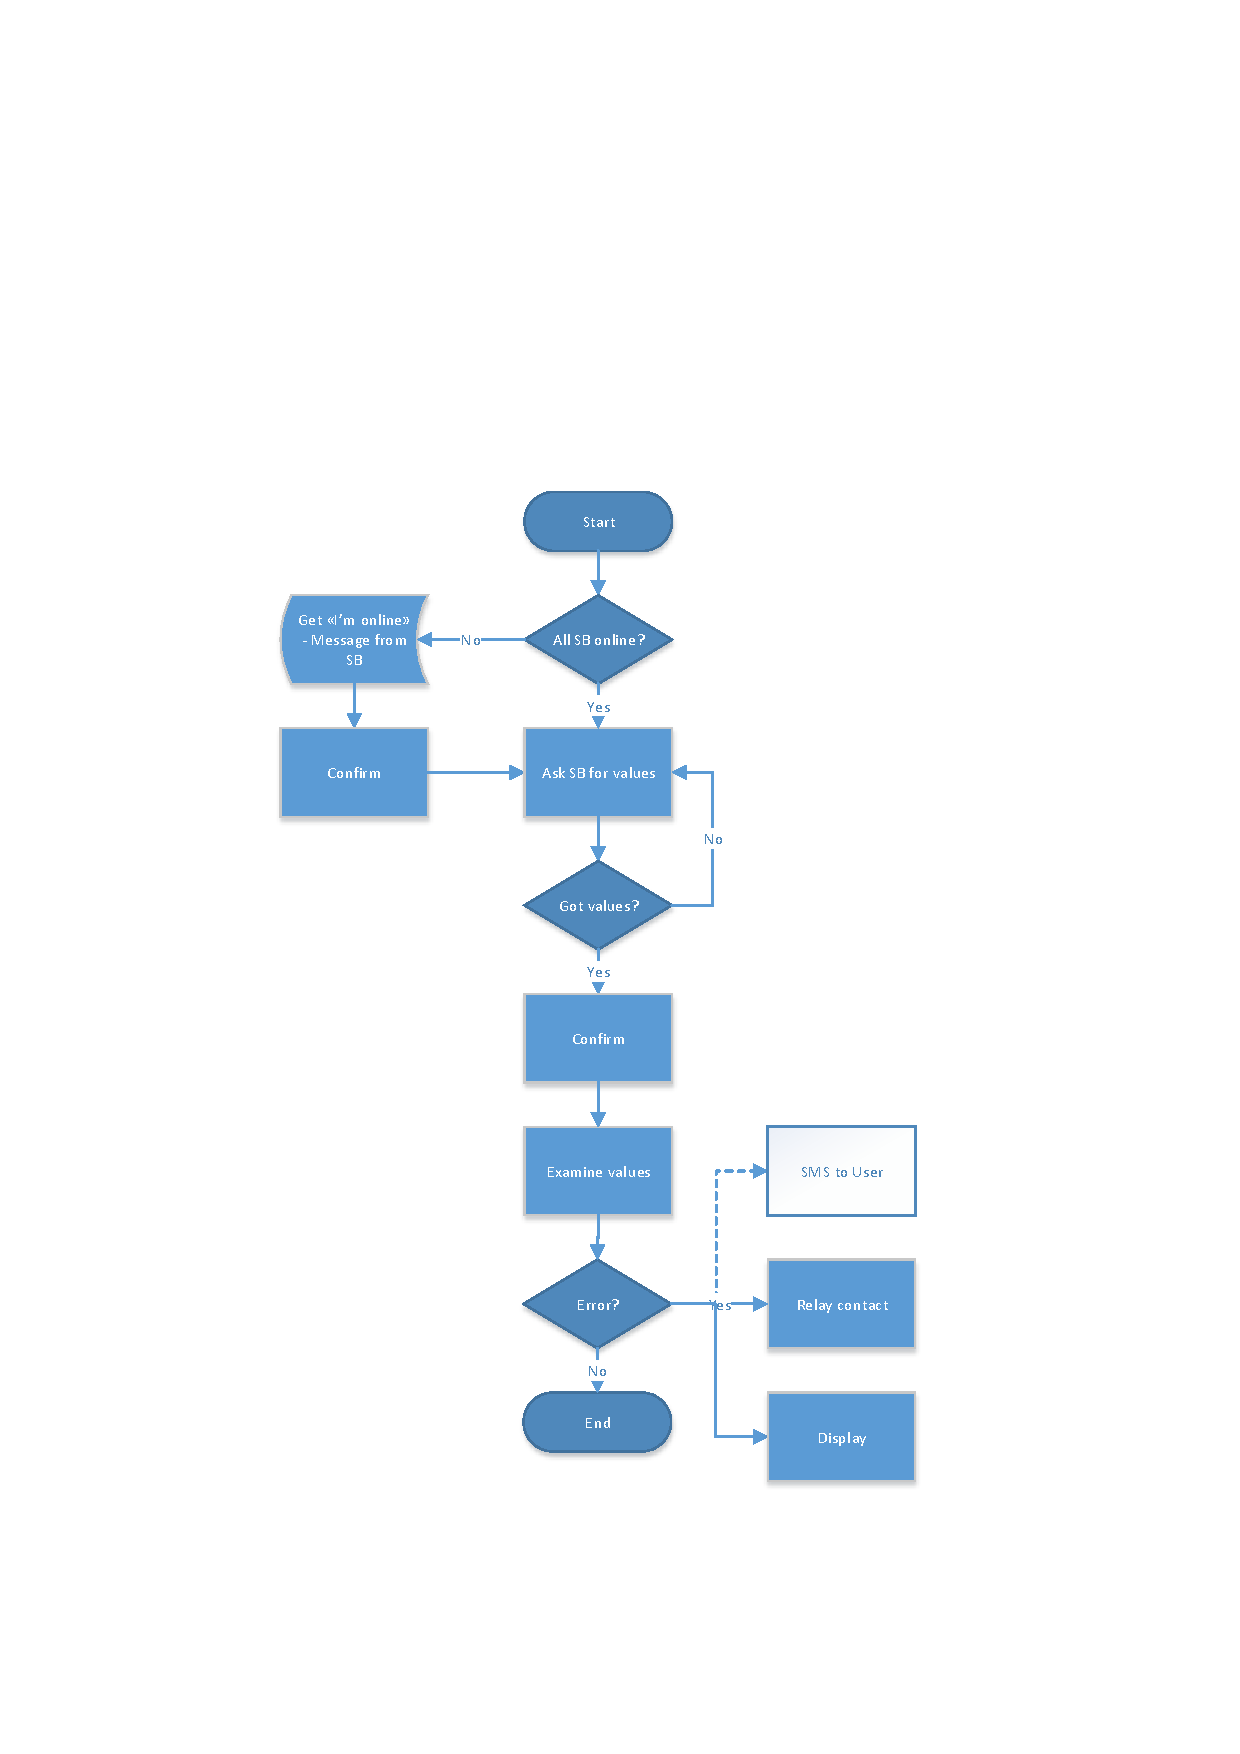
\includegraphics[width=1\textwidth]{graphics/Scheme_report_board}
  \caption{Flussdiagramm Verlauf Programm Meldeplatine}
  \label{fig:Scheme_report_board}
\end{figure}



%\end{document}



